%%%%%%%%%%%%%%%%%%%%%%%%%%%%%%%%%%%%%%%%%%
% Engineering problems / LaTeX Template
%		Semester 5
%		Institut d'Optique Graduate School
%%%%%%%%%%%%%%%%%%%%%%%%%%%%%%%%%%%%%%%%%%
%	5N-OptoElec-Bloc1	/ caractérisation statique
%%%%%%%%%%%%%%%%%%%%%%%%%%%%%%%%%%%%%%%%%%
%
% Created by:
%	Julien VILLEMEJANE - 16/jul/2024
% Modified by: 06/09/24 
%	
%
%%%%%%%%%%%%%%%%%%%%%%%%%%%%%%%%%%%%%%%%%%
% Professional Newsletter Template
% LaTeX Template
% Version 1.0 (09/03/14)
%
% Created by:
% Bob Kerstetter (https://www.tug.org/texshowcase/) and extensively modified by:
% Vel (vel@latextemplates.com)
% 
% This template has been downloaded from:
% http://www.LaTeXTemplates.com
%
% License:
% CC BY-NC-SA 3.0 (http://creativecommons.org/licenses/by-nc-sa/3.0/)
%
%%%%%%%%%%%%%%%%%%%%%%%%%%%%%%%%%%%%%%%%%

\documentclass[a4paper,11pt]{article} % The default font size is 10pt; 11pt and 12pt are alternatives

\usepackage{opto_elec_villemejane}


%%%%%%%%%%%%%%%%%%%%%%%%%%%%%%%%%%%%%%%%%%%%%%%%
%%%%%%%%%%%%%%%%%%%%%%%%%%%%%%%%%%%%%%%%%%%%%%%%
%%%%%%%%%%%%%%%%%%%%%%%%%%%%%%%%%%%%%%%%%%%%%%%%
%%%%%%%%%%%%%%%%%%%%%%%%%%%%%%%%%%%%%%%%%%%%%%%%
\begin{document}


% Page de garde
\begin{titlepage}

\begin{center}
	\begin{minipage}{2.5cm}
	\begin{center}
		
\includegraphics[width=8cm]{images/Logo-LEnsE.png}
	\end{center}
\end{minipage}\hfill
\begin{minipage}{10cm}
	\begin{center}
	\textbf{Institut d'Optique Graduate School }\\[0.1cm]
    \textbf{TP d'Opto-Électronique}


	\end{center}
\end{minipage}\hfill


\vspace{5cm}


{\huge \bfseries \textsc{Opto-Électronique}} \\[0.5cm]
{\large \bfseries Travaux Pratiques} \\[0.2cm]
Semestre 5

\vspace{2cm}
% Title
\rule{\linewidth}{0.3mm} \\[0.4cm]
{ \huge \bfseries\color{violet_iogs} Documentations techniques \\[0.4cm] }
\rule{\linewidth}{0.3mm} \\[1cm]
\end{center}

\vfill

\begin{itemize}
	\item \hyperref[doc:phdSFH206K]{SFH206K}
	\item \hyperref[doc:ledRouge]{LED Rouge}
	\item \hyperref[doc:tl081]{TL081}
	
\end{itemize}


\vfill


\begin{center}
\textit{Les documentations techniques sont disponibles sur le site des constructeurs.}

\end{center}
\end{titlepage}



\titleformat{\section}
  {\null}{}{0pt}{}
  
  

%% Docs techniques
\includepdf[pages=2, pagecommand={\section{\texorpdfstring{\hspace{-1em}}{Doc SFH206K photodiode}}}\label{doc:phdSFH206K}]{ressources/osram_SFH206K.pdf}
\includepdf[pages=4-8]{ressources/osram_SFH206K.pdf}

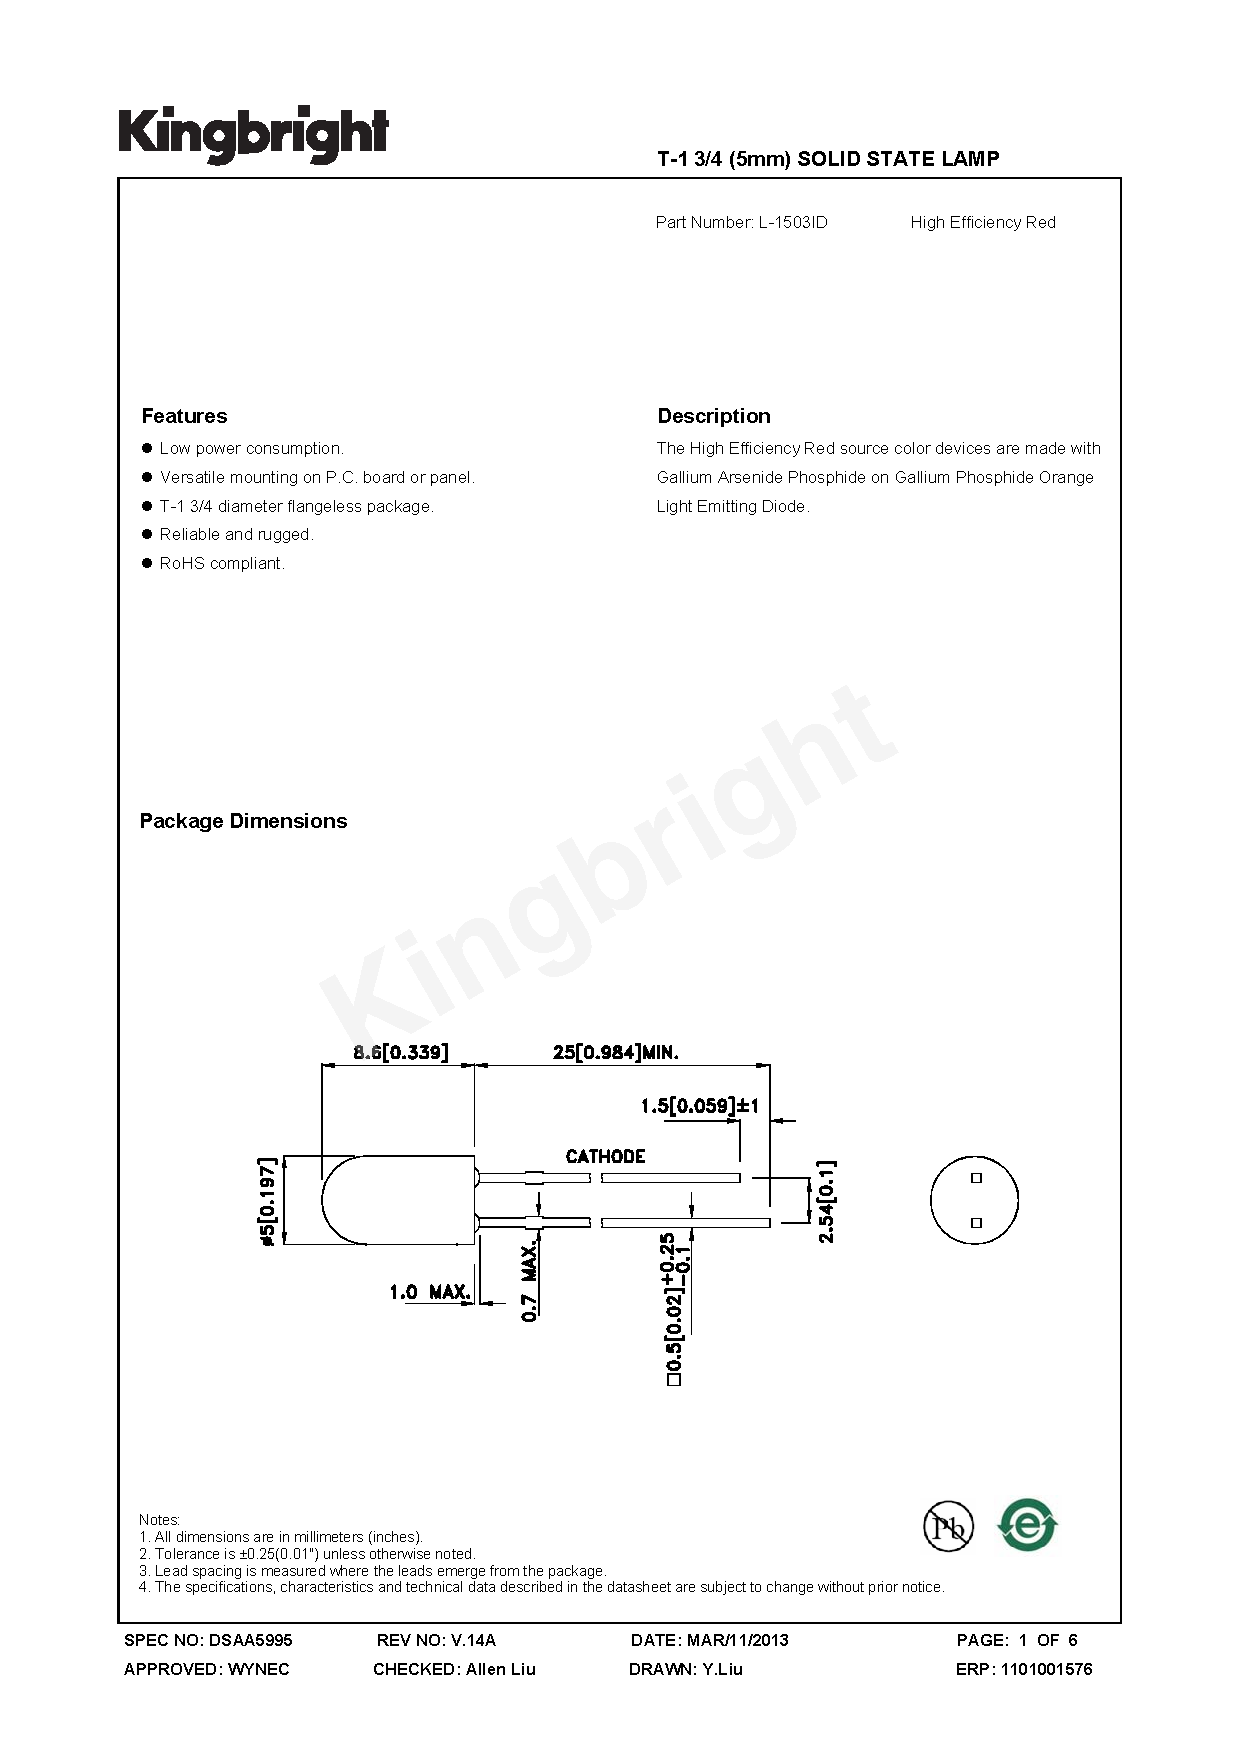
\includepdf[pages=1, pagecommand={\section{\texorpdfstring{\hspace{-1em}}{Doc LED rouge}}}\label{doc:ledRouge}]{ressources/kingbright_LED_Rouge.pdf}
\includepdf[pages={2-3}]{ressources/kingbright_LED_Rouge.pdf}

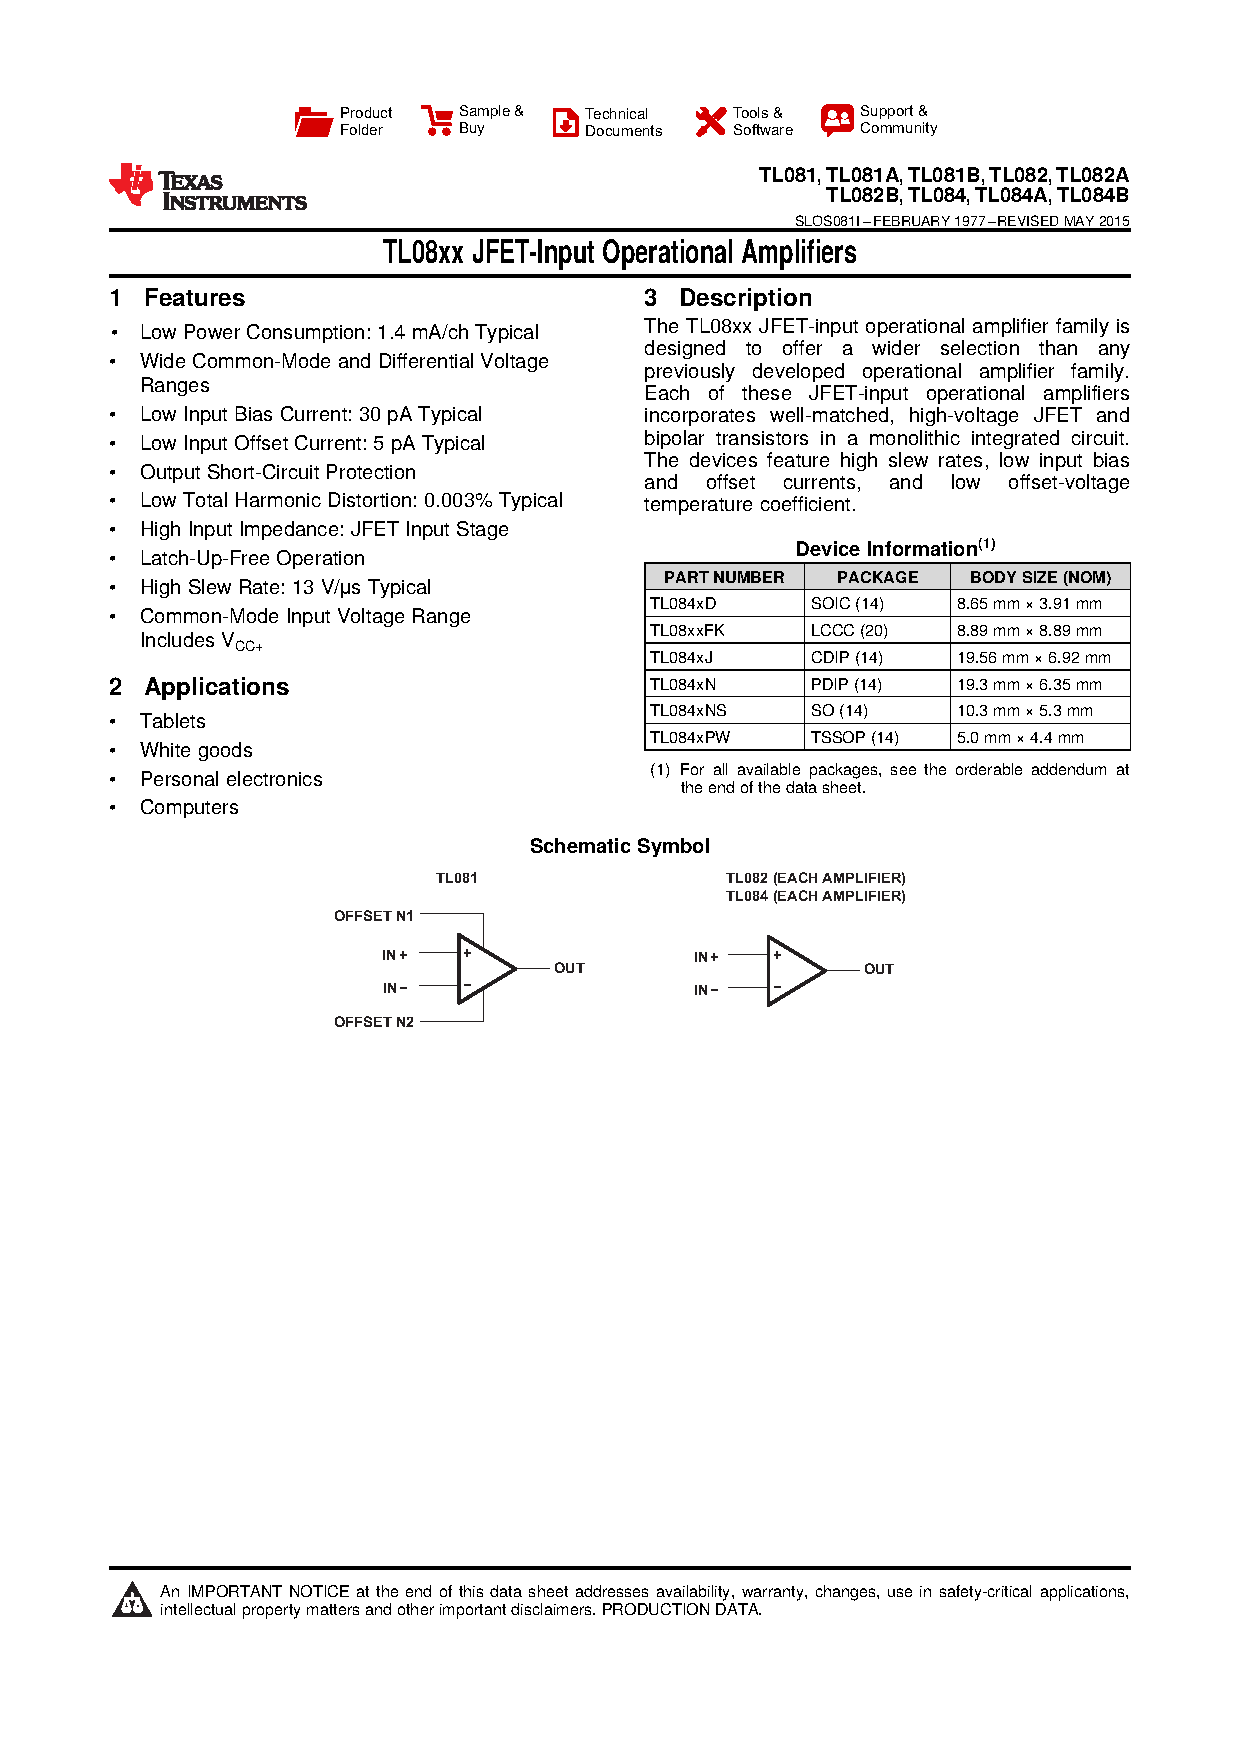
\includepdf[pages=1, pagecommand={\section{\texorpdfstring{\hspace{-1em}}{Doc TL081}}}\label{doc:tl081}]{ressources/tl081.pdf}
\includepdf[pages={2-9}]{ressources/tl081.pdf}

\end{document}


